\documentclass[10pt]{article}
\usepackage{mathtools}
\usepackage{amsfonts}
\usepackage{subcaption} 
\usepackage{url}
\usepackage{gensymb}
\usepackage[a4paper]{geometry}
\usepackage[ampersand]{easylist}
\usepackage{amssymb}
\usepackage{multicol}
\ListProperties(Hide=100, Hang=true, Progressive=3ex, Style*=-- ,
Style2*=$\bullet$ ,Style3*=$\circ$ ,Style4*=\tiny$\blacksquare$ )
\usepackage{graphicx}
\graphicspath{ {images/} }

\begin{document}
\title{
\textsc{Artificial Neural Networks} \\ [20pt]
\huge Benchmark Problems Report \\ % The assignment title
}

\author{Sean Devonport} % Your name

\date{\today} % Today's date or a custom date
\maketitle 

\section{Introduction}
This report is on the performance of neural networks as a tool for modeling data. 4 different data sets have been taken from the UCI Machine Learning database found at \url{http://archive.ics.uci.edu/ml/}. The code was written using Matlab with the help of the neural network toolbox. 

\section{Edibility of Mushrooms}
This data was collected in order to determine the edibility of Agaricus Lepiota mushrooms. It is a supervised classification problem where a mushroom sample is encoded with 22 different features and is then to be classified as either edible or poisonous. 
\subsection{Preprocessing}
The data was provided in file as comma-separated rows of characters. Each column was an feature and each char represented an feature attribute. There was a total of 8124 samples in the data set. The input and target features were encoded using a basic encoding process of converting a particular character into an double. This was done using the Matlab conversion function. Once encoded, the data was transformed into 22xn pattern input and split with  6:2:2 ratio into training, testing and validation sets respectively. The data set was incomplete, any incomplete sample was removed from the set to avoid corrupting the neural net's accuracy for future predictions.

\subsection{Net Performance}
A two-layer scaled conjugate gradient feed forward neural net with backpropogation (SCG) was used. Upon first training of the it was seen that it's performance was extremely satisfactory which didn't warrant much of a need for a experimenting with different architectures. The first layer had 25 neurons and the second had 5. The net trained relatively quickly (under 2min) and had a r and r$^{2}$ values equal to 1 which indicate a perfect classification rate. This was further shown by a mean square error of 0. The figures below show the confusion matrix and classifications  results for training and testing sets activations. 
\newpage

\begin{center}
\begin{figure}[h]
  \begin{subfigure}[b]{0.49\textwidth}
    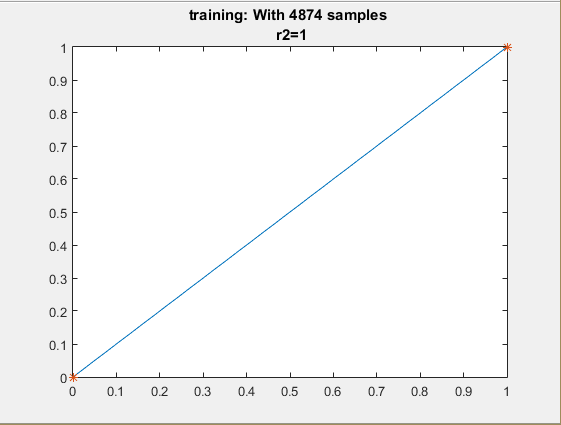
\includegraphics[width=\textwidth]{mush_trainr}
    \caption{Training set with r2=1 }
    \label{fig:1}
  \end{subfigure}
  %
  \begin{subfigure}[b]{0.49\textwidth}
    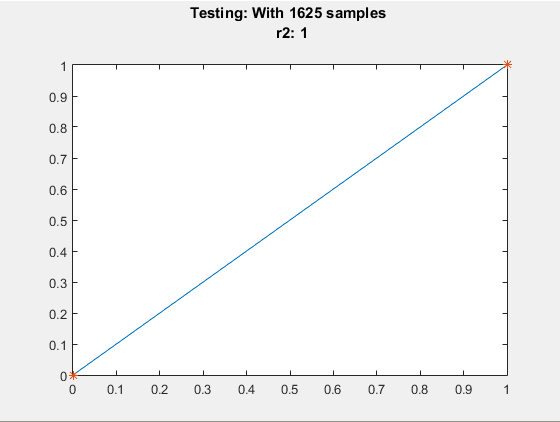
\includegraphics[width=\textwidth]{mush_testr}
    \caption{Testing set with r2=1}
    \label{fig:2}
  \end{subfigure}
  \caption{Linear fit for training and testing outputs vs their targets for mushrooms.}
\end{figure}
\end{center}
These results are extremely promising. We now use the net to simulate on all the mushroom data.
\\

\begin{center}
\begin{figure}[h]
\centering
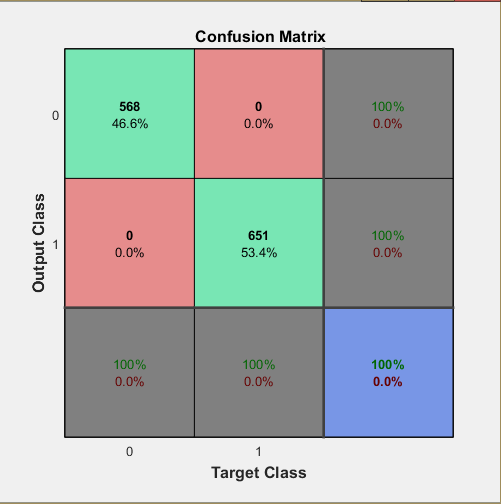
\includegraphics[width=0.49\textwidth]{mush_confusion}
\caption{Confusion matrix for all patterns on the mushroom neural net. We see a 100 percent classification rate}
\end{figure}
\end{center}

The confusion matrix shows that the net has classified all of the mushroom data perfectly. This means that our net is able to be used on new input patterns given to it. Should the user want to simulate on new patterns, they can call \url{mush_fcn.m} on a 22xn column matrix in the same format as the data was originally presented and each sample's edibility will be returned as a 1xn matrix.

\newpage
\section{Origin Cultivars of Wines}
This data was collected to determine the origins of the cultivar of wine based on the wine's chemical composition. It is a supervised classification problem. There are 13 features (alcohol content, malic acid, ash, acalinity of ash, magnesium, total phenols, flavanoids, nonflavanoid phenols, proanthocyanins, color intensity, hue, OD280/OD315 of diluted wines, Proline) which should be used to determine the origin of three different cultivars.
\subsection{Preprocessing}
This data is a complete set with 178 samples. The data has already been presenting in as scalar inputs. The data was separated into 13xn input pattern columns and 1xn target columns and split with a 6:2:2 ratio for training, testing and validation sets, respectively.
\subsection{Net Performance}
A 2-layer SCG net was used. The first layer had 10 neurons and the second 20. These sizes were determined after running a supervising script that determined the optimal layer sizes by selected the net that gave the highest r and r$^{2}$ value. The figures below show the results of this test.
\begin{center}
\begin{figure}[h]
  \begin{subfigure}[b]{0.49\textwidth}
    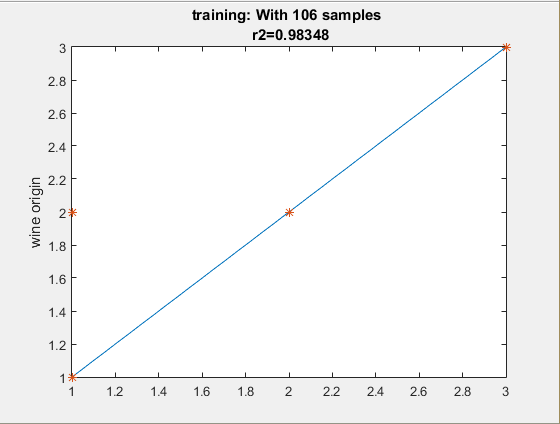
\includegraphics[width=\textwidth]{wine_trainr}
    \caption{Training set with r2=0.98348 }
    \label{fig:1}
  \end{subfigure}
  %
  \begin{subfigure}[b]{0.49\textwidth}
    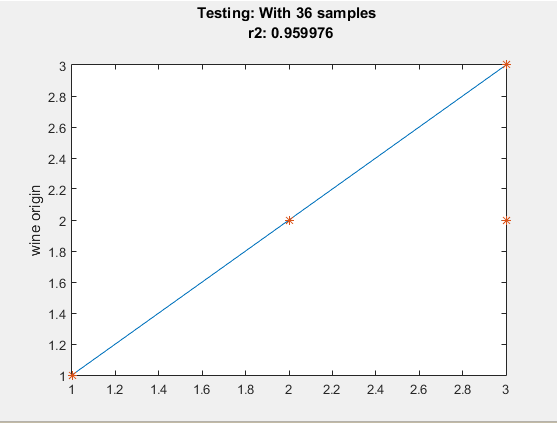
\includegraphics[width=\textwidth]{wine_testr}
    \caption{Testing set with r2=0.959976}
    \label{fig:2}
  \end{subfigure}
  \caption{Training and testing set outputs vs their targets for wine data.}
\end{figure}
\end{center}

These results show a very strong correlation between the net's output and the targets. All the wine data is now simulated on the net. These simulation results show that the net can successfully classify the origin of wines and a function \url{wine_fcn.m} can be called on a 13xn input pattern to get the origin of the wine. 

\begin{center}
\begin{figure}[h]
\centering
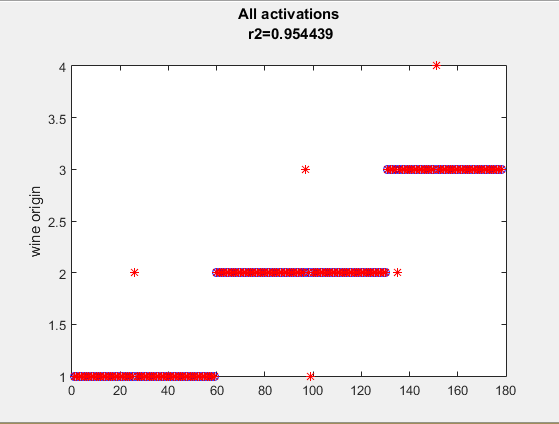
\includegraphics[width=0.49\textwidth]{wine_ar}
\caption{Linear fit for output vs targets of net for all patterns. Asterix denote the net's output.}
\end{figure}
\end{center}

\newpage
\section{Abalone Age}
This data set was collected to determine the age of Abalone based on their physical characteristics. It is a supervised classification problem. There are 8 features (sex, length, diameter, height, whole wight, shucked weight, viscera weight, shell weight, rings) which are used to determine the age of the Abalone.
\subsection{Preprocessing}
This data set was complete and had a total of 4177 samples. The data set required some normalization. The feature column containing the sex of the Abalone has 3 attributes (male, female and infant), these were encoded as 2, 1 and 0 respectively. Once encoded, the features were transformed into 8xn feature columns and their targets encoded as 1xn columns. The data was split with 6:2:2 ratio for training, testing and validation sets, respectively.
\subsection{Net Performance}
Both an SCG net and radial based net were used on this problem but both were unsuccessful in classifying the data correctly.
\\
\\
A supervising script was used which iterated through various layer sizes to determine the most suitable architecture for the net. The net's best effort gave an r$^{2}$ value of 0.565308 on the training set which shows that it did not train successfully. The results on the testing set were not that much better either giving an r$^{2}$ value of 0.60235. Increasing the layer sizes also did not help the net fit the data. In one last attempt a gradient descent training method was used but this too did not yield satisfactory results. This shows that a feed forward net is likely not the best candidate for the job.

\begin{center}
\begin{figure}[h]
\centering
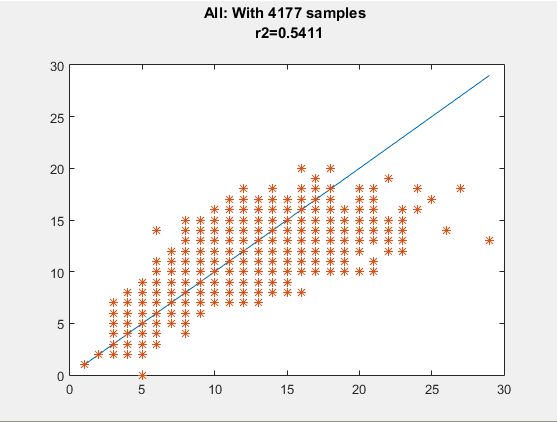
\includegraphics[width=0.50\textwidth]{aba_ar}
\caption{Linear fit for outputs vs their targets Abalone feedforward net. r2 values is 0.5411}
\end{figure}
\end{center}

In attempts to find a net that would solve the problem an RBF net was considered. There were approximately 2000 centres used (half the data set). Various spread sizes were experimented with in an attempt to find one that fits the data best but none were found. The best r$^2$ value for the entire set was 0.398639 so there was almost no correlation. 
\begin{center}
\begin{figure}[h]
\centering
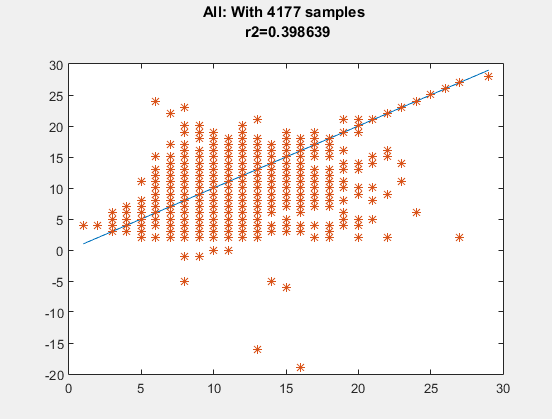
\includegraphics[width=0.50\textwidth]{abarbf_ar}
\caption{Linear fit for outputs vs their targets Abalone RBF net. r2 values is 0.5411}
\end{figure}
\end{center}
It is worth highlighting that the RBF net's training took significantly longer to complete training than the feedforward net. This is due to the large amount of centres used in attempts to train the RBF net.
\\
\\
This data set proved to be difficult to model using feedforward and RBF neural network techniques. This indicates that the age of Abalone may not be able to be determined on physical measurements alone. As the author of the set suggests, further information may be required such as weather patterns, location (which determines food availability etc.) to help increase the chance of creating a model to determine the age of the Abalone.
\newpage
\section{Energy Efficiency}
This data was collected in order to determine the heating and loading requirements of buildings based on their building shape. It is a supervised classification/regression problem. There are 8 features (relative compactness, surface area, wall area, roof area, overall height, orientation, glazing area and glazing area distribution which should determine 2 outcomes, the heating load and cooling load of the building. This should allow architects to be able to design more efficient buildings. 
\subsection{Pre-processing}
The data was complete and required no further sanitizing. There was a total of 768 samples. The data was read in and split into 8xn input pattern features and 2xn target features. The data was split with a 6:2:2 ratio split into training, testing and validation sets respectively. From here, the features are scaled and processed through the net. Matlab's neural network toolbox does this part automatically.
\subsection{Net Performance}
A 2 layer SCG neural net was used. There were 30 neurons in the first layer, and 5 neurons in the second. This architecture was determined after using a supervising script which created multiple 2-layer nets with variable sizes ranging between 5 and 30 with 5 neuron increments from which the net with the highest r and r$^{2}$ value was selected. The figure below shows the correlation results for targets vs outputs of the training and testing sets for the best net.

\begin{center}
\begin{figure}[h]
  \begin{subfigure}[b]{0.49\textwidth}
    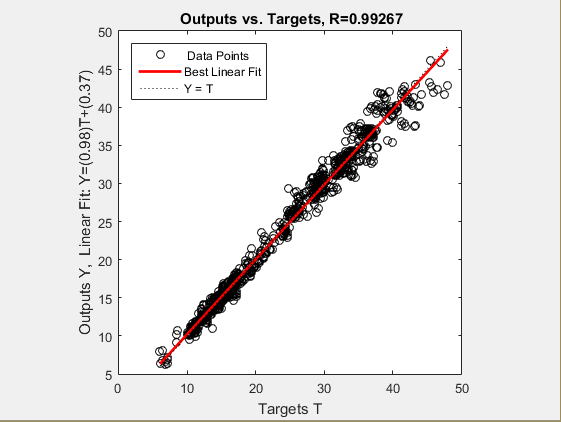
\includegraphics[width=\textwidth]{ee_trainr2}
    \caption{Training set with r2=0.99267 }
    \label{fig:1}
  \end{subfigure}
  %
  \begin{subfigure}[b]{0.49\textwidth}
    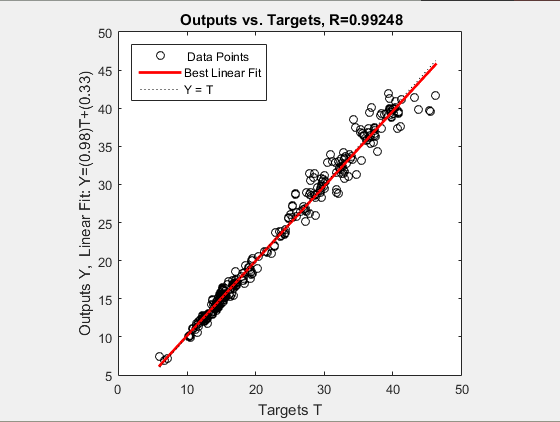
\includegraphics[width=\textwidth]{ee_testr2}
    \caption{Testing set with r2=0.9948}
    \label{fig:2}
  \end{subfigure}
  \caption{Linear Fit for training and testing set targets vs outputs for energy net.}
\end{figure}
\end{center}

These results are satisfactory. The net classifies most of the data correctly however it is not perfect. The r$^{2}$ value for both training and test sets are high which show a strong correlation between the net's output and their targets. We now simulate all of the patterns through the net and get their activations. 


\begin{center}
\begin{figure}[h]
  \begin{subfigure}[b]{0.49\textwidth}
    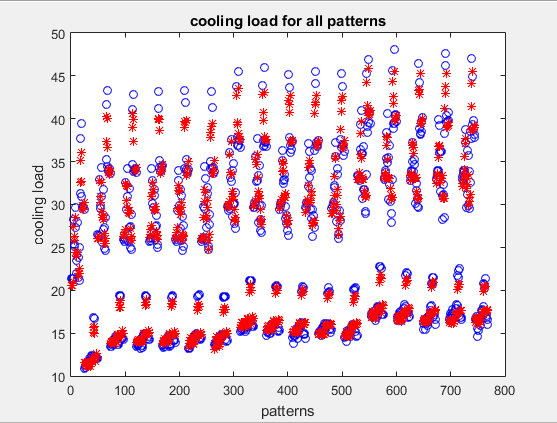
\includegraphics[width=\textwidth]{ee_cl}
    \caption{Cooling load.}
    \label{fig:1}
  \end{subfigure}
  %
  \begin{subfigure}[b]{0.49\textwidth}
    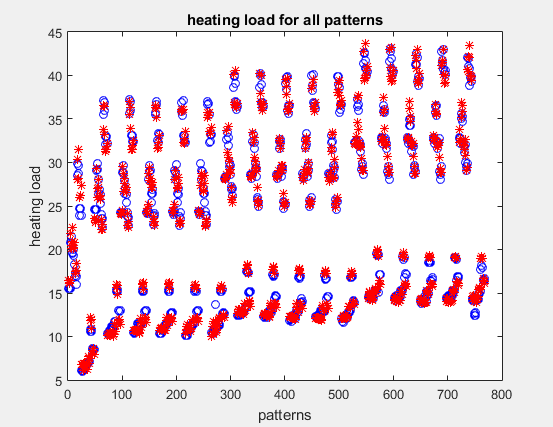
\includegraphics[width=\textwidth]{ee_hl}
    \caption{Heating load.}
    \label{fig:2}
  \end{subfigure}
  \caption{Linear Fit of Outputs vs targets of energy net. Asterix denote the net's output.}
\end{figure}
\end{center}
The net can now be used to successfully interpolate new input data by passing an 8xn pattern into the function \url{energy_fcn.m}. It can also plot trends in the data depending on how a user fixes input through the net. 

\end{document}
